% Options for packages loaded elsewhere
\PassOptionsToPackage{unicode}{hyperref}
\PassOptionsToPackage{hyphens}{url}
%
\documentclass[
]{article}
\usepackage{lmodern}
\usepackage{amssymb,amsmath}
\usepackage{ifxetex,ifluatex}
\ifnum 0\ifxetex 1\fi\ifluatex 1\fi=0 % if pdftex
  \usepackage[T1]{fontenc}
  \usepackage[utf8]{inputenc}
  \usepackage{textcomp} % provide euro and other symbols
\else % if luatex or xetex
  \usepackage{unicode-math}
  \defaultfontfeatures{Scale=MatchLowercase}
  \defaultfontfeatures[\rmfamily]{Ligatures=TeX,Scale=1}
\fi
% Use upquote if available, for straight quotes in verbatim environments
\IfFileExists{upquote.sty}{\usepackage{upquote}}{}
\IfFileExists{microtype.sty}{% use microtype if available
  \usepackage[]{microtype}
  \UseMicrotypeSet[protrusion]{basicmath} % disable protrusion for tt fonts
}{}
\makeatletter
\@ifundefined{KOMAClassName}{% if non-KOMA class
  \IfFileExists{parskip.sty}{%
    \usepackage{parskip}
  }{% else
    \setlength{\parindent}{0pt}
    \setlength{\parskip}{6pt plus 2pt minus 1pt}}
}{% if KOMA class
  \KOMAoptions{parskip=half}}
\makeatother
\usepackage{xcolor}
\IfFileExists{xurl.sty}{\usepackage{xurl}}{} % add URL line breaks if available
\IfFileExists{bookmark.sty}{\usepackage{bookmark}}{\usepackage{hyperref}}
\hypersetup{
  pdftitle={622\_HW1},
  hidelinks,
  pdfcreator={LaTeX via pandoc}}
\urlstyle{same} % disable monospaced font for URLs
\usepackage[margin=1in]{geometry}
\usepackage{color}
\usepackage{fancyvrb}
\newcommand{\VerbBar}{|}
\newcommand{\VERB}{\Verb[commandchars=\\\{\}]}
\DefineVerbatimEnvironment{Highlighting}{Verbatim}{commandchars=\\\{\}}
% Add ',fontsize=\small' for more characters per line
\usepackage{framed}
\definecolor{shadecolor}{RGB}{248,248,248}
\newenvironment{Shaded}{\begin{snugshade}}{\end{snugshade}}
\newcommand{\AlertTok}[1]{\textcolor[rgb]{0.94,0.16,0.16}{#1}}
\newcommand{\AnnotationTok}[1]{\textcolor[rgb]{0.56,0.35,0.01}{\textbf{\textit{#1}}}}
\newcommand{\AttributeTok}[1]{\textcolor[rgb]{0.77,0.63,0.00}{#1}}
\newcommand{\BaseNTok}[1]{\textcolor[rgb]{0.00,0.00,0.81}{#1}}
\newcommand{\BuiltInTok}[1]{#1}
\newcommand{\CharTok}[1]{\textcolor[rgb]{0.31,0.60,0.02}{#1}}
\newcommand{\CommentTok}[1]{\textcolor[rgb]{0.56,0.35,0.01}{\textit{#1}}}
\newcommand{\CommentVarTok}[1]{\textcolor[rgb]{0.56,0.35,0.01}{\textbf{\textit{#1}}}}
\newcommand{\ConstantTok}[1]{\textcolor[rgb]{0.00,0.00,0.00}{#1}}
\newcommand{\ControlFlowTok}[1]{\textcolor[rgb]{0.13,0.29,0.53}{\textbf{#1}}}
\newcommand{\DataTypeTok}[1]{\textcolor[rgb]{0.13,0.29,0.53}{#1}}
\newcommand{\DecValTok}[1]{\textcolor[rgb]{0.00,0.00,0.81}{#1}}
\newcommand{\DocumentationTok}[1]{\textcolor[rgb]{0.56,0.35,0.01}{\textbf{\textit{#1}}}}
\newcommand{\ErrorTok}[1]{\textcolor[rgb]{0.64,0.00,0.00}{\textbf{#1}}}
\newcommand{\ExtensionTok}[1]{#1}
\newcommand{\FloatTok}[1]{\textcolor[rgb]{0.00,0.00,0.81}{#1}}
\newcommand{\FunctionTok}[1]{\textcolor[rgb]{0.00,0.00,0.00}{#1}}
\newcommand{\ImportTok}[1]{#1}
\newcommand{\InformationTok}[1]{\textcolor[rgb]{0.56,0.35,0.01}{\textbf{\textit{#1}}}}
\newcommand{\KeywordTok}[1]{\textcolor[rgb]{0.13,0.29,0.53}{\textbf{#1}}}
\newcommand{\NormalTok}[1]{#1}
\newcommand{\OperatorTok}[1]{\textcolor[rgb]{0.81,0.36,0.00}{\textbf{#1}}}
\newcommand{\OtherTok}[1]{\textcolor[rgb]{0.56,0.35,0.01}{#1}}
\newcommand{\PreprocessorTok}[1]{\textcolor[rgb]{0.56,0.35,0.01}{\textit{#1}}}
\newcommand{\RegionMarkerTok}[1]{#1}
\newcommand{\SpecialCharTok}[1]{\textcolor[rgb]{0.00,0.00,0.00}{#1}}
\newcommand{\SpecialStringTok}[1]{\textcolor[rgb]{0.31,0.60,0.02}{#1}}
\newcommand{\StringTok}[1]{\textcolor[rgb]{0.31,0.60,0.02}{#1}}
\newcommand{\VariableTok}[1]{\textcolor[rgb]{0.00,0.00,0.00}{#1}}
\newcommand{\VerbatimStringTok}[1]{\textcolor[rgb]{0.31,0.60,0.02}{#1}}
\newcommand{\WarningTok}[1]{\textcolor[rgb]{0.56,0.35,0.01}{\textbf{\textit{#1}}}}
\usepackage{graphicx,grffile}
\makeatletter
\def\maxwidth{\ifdim\Gin@nat@width>\linewidth\linewidth\else\Gin@nat@width\fi}
\def\maxheight{\ifdim\Gin@nat@height>\textheight\textheight\else\Gin@nat@height\fi}
\makeatother
% Scale images if necessary, so that they will not overflow the page
% margins by default, and it is still possible to overwrite the defaults
% using explicit options in \includegraphics[width, height, ...]{}
\setkeys{Gin}{width=\maxwidth,height=\maxheight,keepaspectratio}
% Set default figure placement to htbp
\makeatletter
\def\fps@figure{htbp}
\makeatother
\setlength{\emergencystretch}{3em} % prevent overfull lines
\providecommand{\tightlist}{%
  \setlength{\itemsep}{0pt}\setlength{\parskip}{0pt}}
\setcounter{secnumdepth}{-\maxdimen} % remove section numbering
\usepackage{booktabs}
\usepackage{longtable}
\usepackage{array}
\usepackage{multirow}
\usepackage{wrapfig}
\usepackage{float}
\usepackage{colortbl}
\usepackage{pdflscape}
\usepackage{tabu}
\usepackage{threeparttable}
\usepackage{threeparttablex}
\usepackage[normalem]{ulem}
\usepackage{makecell}

\title{622\_HW1}
\author{}
\date{\vspace{-2.5em}}

\begin{document}
\maketitle

\begin{Shaded}
\begin{Highlighting}[]
\KeywordTok{library}\NormalTok{(naivebayes)}
\KeywordTok{library}\NormalTok{(class)}
\KeywordTok{library}\NormalTok{(gmodels)}
\KeywordTok{library}\NormalTok{(tidyverse)}
\KeywordTok{library}\NormalTok{(caret)}
\KeywordTok{library}\NormalTok{(pROC)}
\KeywordTok{library}\NormalTok{(kableExtra)}
\KeywordTok{library}\NormalTok{(class)}
\KeywordTok{library}\NormalTok{(ROCR)}
\end{Highlighting}
\end{Shaded}

\begin{Shaded}
\begin{Highlighting}[]
\NormalTok{df <-}\StringTok{ }\KeywordTok{read.csv}\NormalTok{(}\StringTok{'HW1.csv'}\NormalTok{, }\DataTypeTok{header =} \OtherTok{TRUE}\NormalTok{)}
\NormalTok{df}\OperatorTok{$}\NormalTok{label <-}\StringTok{ }\KeywordTok{as.factor}\NormalTok{(df}\OperatorTok{$}\NormalTok{label)}
\NormalTok{df}\OperatorTok{$}\NormalTok{Y <-}\StringTok{ }\KeywordTok{as.factor}\NormalTok{(df}\OperatorTok{$}\NormalTok{Y)}

\KeywordTok{summary}\NormalTok{(df)}
\end{Highlighting}
\end{Shaded}

\begin{verbatim}
##        X      Y       label   
##  Min.   : 5   a:6   BLACK:22  
##  1st Qu.:19   b:6   BLUE :14  
##  Median :43   c:6             
##  Mean   :38   d:6             
##  3rd Qu.:55   e:6             
##  Max.   :63   f:6
\end{verbatim}

\begin{Shaded}
\begin{Highlighting}[]
\KeywordTok{str}\NormalTok{(df)}
\end{Highlighting}
\end{Shaded}

\begin{verbatim}
## 'data.frame':    36 obs. of  3 variables:
##  $ X    : int  5 5 5 5 5 5 19 19 19 19 ...
##  $ Y    : Factor w/ 6 levels "a","b","c","d",..: 1 2 3 4 5 6 1 2 3 4 ...
##  $ label: Factor w/ 2 levels "BLACK","BLUE": 2 1 2 1 1 1 2 2 2 2 ...
\end{verbatim}

\begin{Shaded}
\begin{Highlighting}[]
\KeywordTok{head}\NormalTok{(df)}
\end{Highlighting}
\end{Shaded}

\begin{verbatim}
##   X Y label
## 1 5 a  BLUE
## 2 5 b BLACK
## 3 5 c  BLUE
## 4 5 d BLACK
## 5 5 e BLACK
## 6 5 f BLACK
\end{verbatim}

\hypertarget{explorative-data-analysis}{%
\subsection{Explorative Data Analysis}\label{explorative-data-analysis}}

\begin{Shaded}
\begin{Highlighting}[]
\NormalTok{df }\OperatorTok\StringTok{ }\KeywordTok{ggplot}\NormalTok{(}\KeywordTok{aes}\NormalTok{(}\DataTypeTok{x=}\NormalTok{label)) }\OperatorTok{+}
\StringTok{        }\KeywordTok{geom_bar}\NormalTok{() }\OperatorTok{+}
\StringTok{  }\KeywordTok{ggtitle}\NormalTok{(}\StringTok{"Label distribution Plot"}\NormalTok{)}
\end{Highlighting}
\end{Shaded}

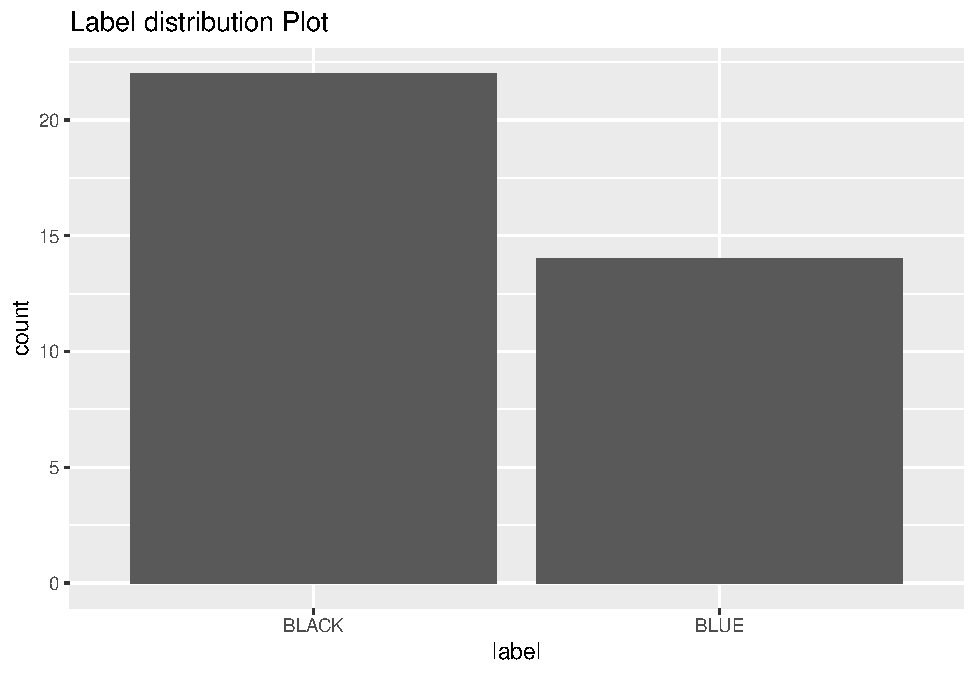
\includegraphics{622_HW1_files/figure-latex/unnamed-chunk-3-1.pdf}

\begin{Shaded}
\begin{Highlighting}[]
\NormalTok{df }\OperatorTok\StringTok{ }\KeywordTok{ggplot}\NormalTok{(}\KeywordTok{aes}\NormalTok{(}\DataTypeTok{x=}\NormalTok{Y)) }\OperatorTok{+}
\StringTok{        }\KeywordTok{geom_bar}\NormalTok{() }\OperatorTok{+}
\StringTok{  }\KeywordTok{ggtitle}\NormalTok{(}\StringTok{"Y distribution Plot"}\NormalTok{)}
\end{Highlighting}
\end{Shaded}

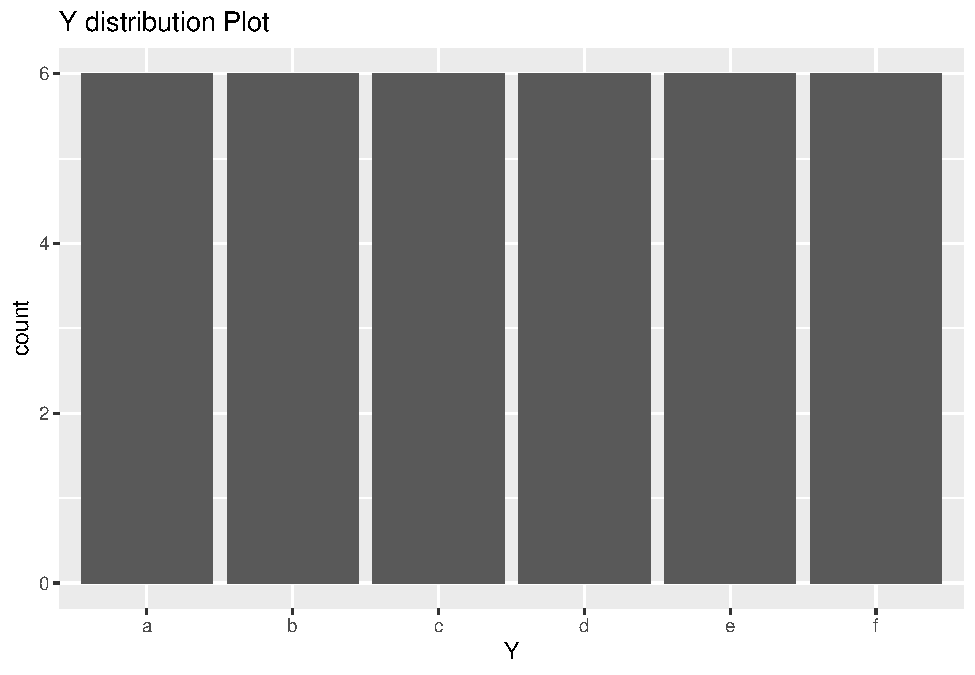
\includegraphics{622_HW1_files/figure-latex/unnamed-chunk-3-2.pdf}

\begin{Shaded}
\begin{Highlighting}[]
\NormalTok{df }\OperatorTok\StringTok{ }\KeywordTok{ggplot}\NormalTok{(}\KeywordTok{aes}\NormalTok{(}\DataTypeTok{x=}\NormalTok{X)) }\OperatorTok{+}
\StringTok{        }\KeywordTok{geom_bar}\NormalTok{() }\OperatorTok{+}
\StringTok{  }\KeywordTok{ggtitle}\NormalTok{(}\StringTok{"X distribution Plot"}\NormalTok{)}
\end{Highlighting}
\end{Shaded}

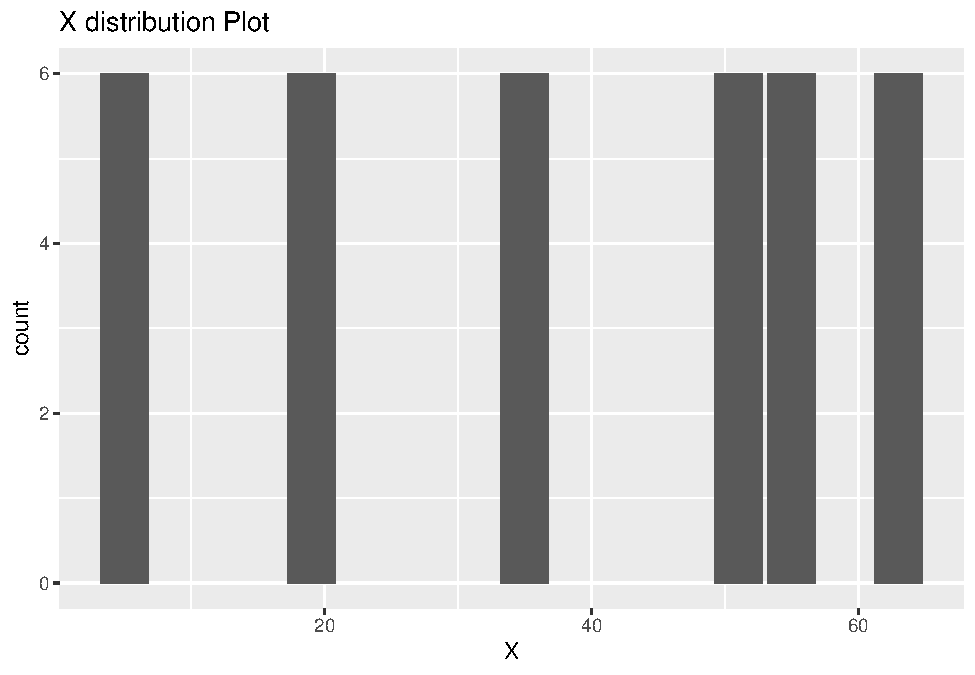
\includegraphics{622_HW1_files/figure-latex/unnamed-chunk-3-3.pdf}

\begin{Shaded}
\begin{Highlighting}[]
\KeywordTok{ggplot}\NormalTok{() }\OperatorTok{+}\StringTok{ }\KeywordTok{geom_point}\NormalTok{(}\DataTypeTok{data =}\NormalTok{ df, }\KeywordTok{aes}\NormalTok{(}\DataTypeTok{x =}\NormalTok{ Y, }\DataTypeTok{y =}\NormalTok{ X, }\DataTypeTok{color =}\NormalTok{ label), }\DataTypeTok{size=}\DecValTok{3}\NormalTok{) }\OperatorTok{+}\StringTok{ }\KeywordTok{ggtitle}\NormalTok{(}\StringTok{"Scatter Plot b/w X and Y"}\NormalTok{)}
\end{Highlighting}
\end{Shaded}

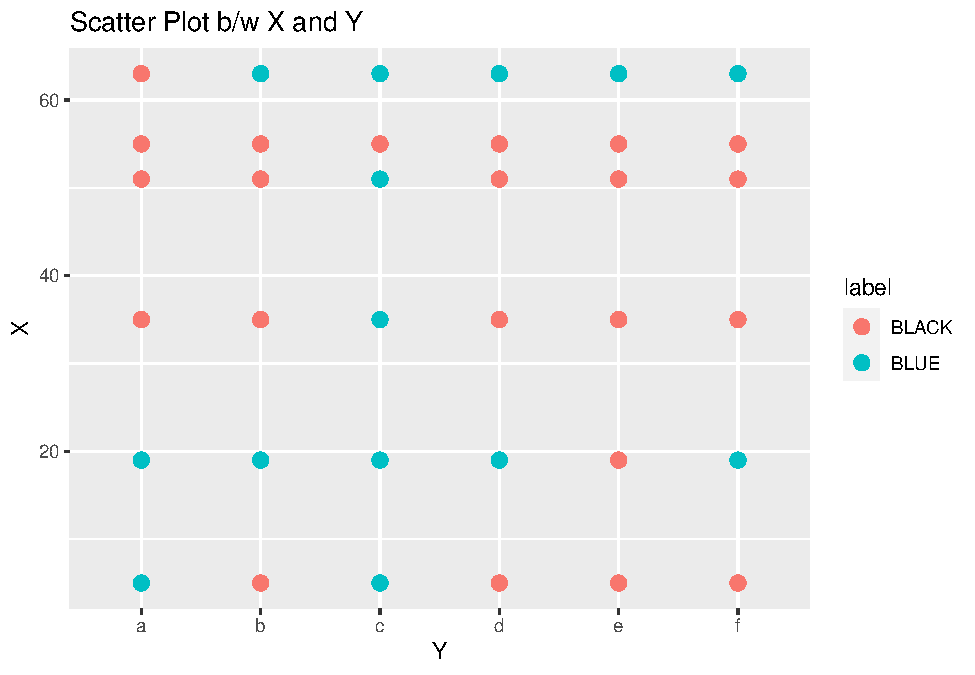
\includegraphics{622_HW1_files/figure-latex/unnamed-chunk-3-4.pdf}

\hypertarget{correlation-variables}{%
\subsection{\texorpdfstring{\textbf{Correlation
variables}}{Correlation variables}}\label{correlation-variables}}

\begin{Shaded}
\begin{Highlighting}[]
\KeywordTok{pairs}\NormalTok{(df)}
\end{Highlighting}
\end{Shaded}

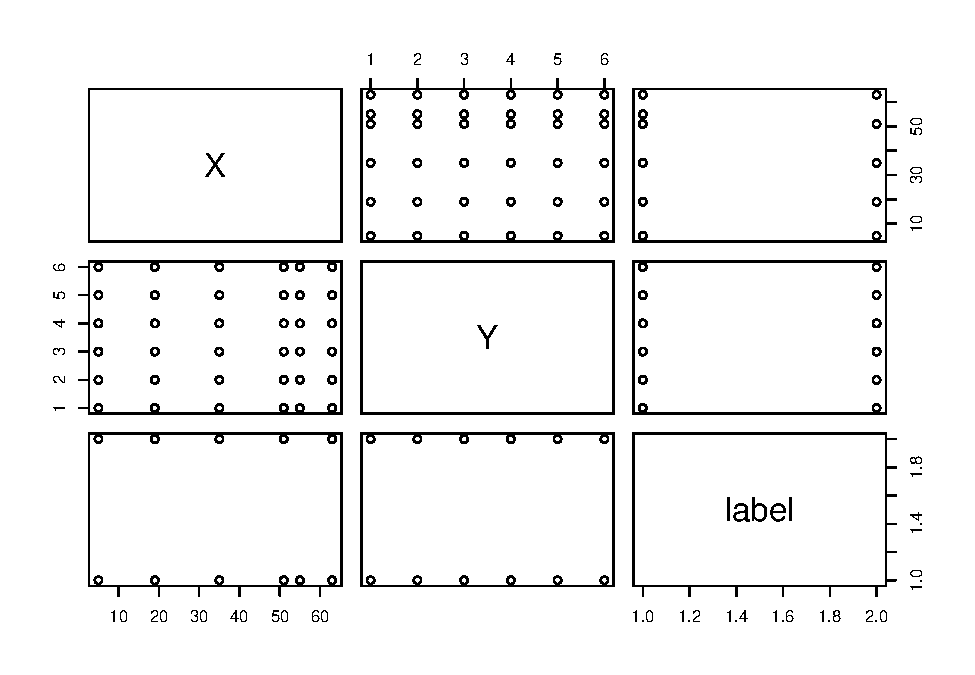
\includegraphics{622_HW1_files/figure-latex/unnamed-chunk-4-1.pdf}

\hypertarget{split-the-data}{%
\subsection{\texorpdfstring{\textbf{Split the
data}}{Split the data}}\label{split-the-data}}

\begin{Shaded}
\begin{Highlighting}[]
\KeywordTok{set.seed}\NormalTok{(}\DecValTok{1234}\NormalTok{)}

\NormalTok{ind <-}\StringTok{ }\KeywordTok{sample}\NormalTok{(}\DecValTok{2}\NormalTok{, }\KeywordTok{nrow}\NormalTok{(df), }\DataTypeTok{replace =}\NormalTok{ T, }\DataTypeTok{prob=}\KeywordTok{c}\NormalTok{(}\FloatTok{0.7}\NormalTok{,}\FloatTok{0.3}\NormalTok{))}
\NormalTok{train <-}\StringTok{ }\NormalTok{df[ind }\OperatorTok{==}\DecValTok{1}\NormalTok{,]}
\NormalTok{test <-}\StringTok{ }\NormalTok{df[ind}\OperatorTok{==}\DecValTok{2}\NormalTok{,]}

\NormalTok{train}
\end{Highlighting}
\end{Shaded}

\begin{verbatim}
##     X Y label
## 1   5 a  BLUE
## 2   5 b BLACK
## 3   5 c  BLUE
## 4   5 d BLACK
## 6   5 f BLACK
## 7  19 a  BLUE
## 8  19 b  BLUE
## 9  19 c  BLUE
## 10 19 d  BLUE
## 11 19 e BLACK
## 12 19 f  BLUE
## 13 35 a BLACK
## 15 35 c  BLUE
## 17 35 e BLACK
## 18 35 f BLACK
## 19 51 a BLACK
## 20 51 b BLACK
## 21 51 c  BLUE
## 22 51 d BLACK
## 23 51 e BLACK
## 24 51 f BLACK
## 25 55 a BLACK
## 27 55 c BLACK
## 30 55 f BLACK
## 31 63 a BLACK
## 32 63 b  BLUE
## 33 63 c  BLUE
## 34 63 d  BLUE
## 35 63 e  BLUE
\end{verbatim}

\begin{Shaded}
\begin{Highlighting}[]
\NormalTok{test}
\end{Highlighting}
\end{Shaded}

\begin{verbatim}
##     X Y label
## 5   5 e BLACK
## 14 35 b BLACK
## 16 35 d BLACK
## 26 55 b BLACK
## 28 55 d BLACK
## 29 55 e BLACK
## 36 63 f  BLUE
\end{verbatim}

\hypertarget{naivebayes-classifier}{%
\subsection{\texorpdfstring{\textbf{NaiveBayes
Classifier}}{NaiveBayes Classifier}}\label{naivebayes-classifier}}

\begin{Shaded}
\begin{Highlighting}[]
\NormalTok{nb_model <-}\StringTok{ }\KeywordTok{naive_bayes}\NormalTok{(label}\OperatorTok{~}\NormalTok{., }\DataTypeTok{data=}\NormalTok{df)}
\KeywordTok{summary}\NormalTok{(nb_model)}
\end{Highlighting}
\end{Shaded}

\begin{verbatim}
## 
## ================================== Naive Bayes ================================== 
##  
## - Call: naive_bayes.formula(formula = label ~ ., data = df) 
## - Laplace: 0 
## - Classes: 2 
## - Samples: 36 
## - Features: 2 
## - Conditional distributions: 
##     - Categorical: 1
##     - Gaussian: 1
## - Prior probabilities: 
##     - BLACK: 0.6111
##     - BLUE: 0.3889
## 
## ---------------------------------------------------------------------------------
\end{verbatim}

\begin{Shaded}
\begin{Highlighting}[]
\NormalTok{trainPredict <-}\StringTok{ }\KeywordTok{predict}\NormalTok{(nb_model, train)}

\CommentTok{#ConfusionMatrix on Train data}
\NormalTok{ConfusionMatrix <-}\StringTok{ }\KeywordTok{table}\NormalTok{(trainPredict, train}\OperatorTok{$}\NormalTok{label)}
\NormalTok{ConfusionMatrix}
\end{Highlighting}
\end{Shaded}

\begin{verbatim}
##             
## trainPredict BLACK BLUE
##        BLACK    15    8
##        BLUE      1    5
\end{verbatim}

\begin{Shaded}
\begin{Highlighting}[]
\NormalTok{model_metrics_df <-}\StringTok{ }\KeywordTok{data.frame}\NormalTok{(}\DataTypeTok{Type=}\OtherTok{NA}\NormalTok{, }\DataTypeTok{Algo=}\OtherTok{NA}\NormalTok{, }\DataTypeTok{AUC=}\OtherTok{NA}\NormalTok{, }\DataTypeTok{ACCURACY=}\OtherTok{NA}\NormalTok{,}\DataTypeTok{TPR=}\OtherTok{NA}\NormalTok{,}\DataTypeTok{FPR=}\OtherTok{NA}\NormalTok{,}\DataTypeTok{TNR=}\OtherTok{NA}\NormalTok{,}\DataTypeTok{FNR=}\OtherTok{NA}\NormalTok{)}

\NormalTok{model_metrics_df <-}\StringTok{ }\KeywordTok{gather_metrics_func}\NormalTok{(}\StringTok{'Train'}\NormalTok{, model_metrics_df, }\StringTok{'NB'}\NormalTok{,trainPredict, train)}

\NormalTok{testPredict <-}\StringTok{ }\KeywordTok{predict}\NormalTok{(nb_model, test)}

\CommentTok{#ConfusionMatrix on Test data}
\NormalTok{ConfusionMatrix <-}\StringTok{ }\KeywordTok{table}\NormalTok{(testPredict, test}\OperatorTok{$}\NormalTok{label)}
\NormalTok{ConfusionMatrix}
\end{Highlighting}
\end{Shaded}

\begin{verbatim}
##            
## testPredict BLACK BLUE
##       BLACK     6    1
##       BLUE      0    0
\end{verbatim}

\begin{Shaded}
\begin{Highlighting}[]
\NormalTok{model_metrics_df <-}\StringTok{ }\KeywordTok{gather_metrics_func}\NormalTok{(}\StringTok{'Test'}\NormalTok{, model_metrics_df, }\StringTok{'NB'}\NormalTok{,testPredict, test)}
\end{Highlighting}
\end{Shaded}

\hypertarget{since-the-model-is-successfully-predicting-values-on-test-dataseti.e.-new-dataunseen-data-more-than-training-set-accuracy-we-can-say-that-it-is-generalizable.}{%
\paragraph{\texorpdfstring{\textbf{Since the model is successfully
predicting values on test dataset(i.e., new data/unseen data) more than
training set accuracy, we can say that it is
generalizable.}}{Since the model is successfully predicting values on test dataset(i.e., new data/unseen data) more than training set accuracy, we can say that it is generalizable.}}\label{since-the-model-is-successfully-predicting-values-on-test-dataseti.e.-new-dataunseen-data-more-than-training-set-accuracy-we-can-say-that-it-is-generalizable.}}

\hypertarget{logistic-regression}{%
\subsection{\texorpdfstring{\textbf{Logistic
Regression}}{Logistic Regression}}\label{logistic-regression}}

\begin{Shaded}
\begin{Highlighting}[]
\NormalTok{lm_model <-}\StringTok{ }\KeywordTok{glm}\NormalTok{(label}\OperatorTok{~}\NormalTok{., }\DataTypeTok{data=}\NormalTok{train, }\DataTypeTok{family=}\KeywordTok{binomial}\NormalTok{(}\DataTypeTok{link=}\StringTok{"logit"}\NormalTok{))}
\KeywordTok{summary}\NormalTok{(lm_model)}
\end{Highlighting}
\end{Shaded}

\begin{verbatim}
## 
## Call:
## glm(formula = label ~ ., family = binomial(link = "logit"), data = train)
## 
## Deviance Residuals: 
##     Min       1Q   Median       3Q      Max  
## -1.7967  -0.8274  -0.5873   1.0835   1.8081  
## 
## Coefficients:
##             Estimate Std. Error z value Pr(>|z|)  
## (Intercept) -0.15613    1.14121  -0.137   0.8912  
## X           -0.01451    0.02031  -0.714   0.4751  
## Yb           0.65673    1.33991   0.490   0.6240  
## Yc           2.34610    1.41185   1.662   0.0966 .
## Yd           0.65673    1.33991   0.490   0.6240  
## Ye          -0.34758    1.45593  -0.239   0.8113  
## Yf          -0.77402    1.43062  -0.541   0.5885  
## ---
## Signif. codes:  0 '***' 0.001 '**' 0.01 '*' 0.05 '.' 0.1 ' ' 1
## 
## (Dispersion parameter for binomial family taken to be 1)
## 
##     Null deviance: 39.892  on 28  degrees of freedom
## Residual deviance: 33.119  on 22  degrees of freedom
## AIC: 47.119
## 
## Number of Fisher Scoring iterations: 4
\end{verbatim}

\begin{Shaded}
\begin{Highlighting}[]
\NormalTok{predict_lr_train <-}\StringTok{ }\KeywordTok{predict}\NormalTok{(lm_model, }\DataTypeTok{newdata=}\NormalTok{train, }\DataTypeTok{type =} \StringTok{"response"}\NormalTok{)}
\NormalTok{predict_lr_train<-}\StringTok{ }\KeywordTok{ifelse}\NormalTok{(predict_lr_train}\OperatorTok{<}\FloatTok{0.5}\NormalTok{,}\StringTok{"BLACK"}\NormalTok{,}\StringTok{"BLUE"}\NormalTok{ )}
\NormalTok{predict_lr_train <-}\StringTok{ }\KeywordTok{as.factor}\NormalTok{(predict_lr_train)}

\NormalTok{model_metrics_df <-}\StringTok{ }\KeywordTok{gather_metrics_func}\NormalTok{(}\StringTok{'Train'}\NormalTok{, model_metrics_df, }\StringTok{'LR'}\NormalTok{,predict_lr_train, train)}

\NormalTok{predict_lr_test <-}\StringTok{ }\KeywordTok{predict}\NormalTok{(lm_model, }\DataTypeTok{newdata=}\NormalTok{test, }\DataTypeTok{type =} \StringTok{"response"}\NormalTok{)}
\NormalTok{predict_lr_test<-}\StringTok{ }\KeywordTok{ifelse}\NormalTok{(predict_lr_test}\OperatorTok{<}\FloatTok{0.5}\NormalTok{,}\StringTok{"BLACK"}\NormalTok{,}\StringTok{"BLUE"}\NormalTok{ )}
\NormalTok{predict_lr_test <-}\StringTok{ }\KeywordTok{as.factor}\NormalTok{(predict_lr_test)}

\NormalTok{model_metrics_df <-}\StringTok{ }\KeywordTok{gather_metrics_func}\NormalTok{(}\StringTok{'Test'}\NormalTok{, model_metrics_df, }\StringTok{'LR'}\NormalTok{,predict_lr_test, test)}
\end{Highlighting}
\end{Shaded}

\hypertarget{knn---3}{%
\subsection{\texorpdfstring{\textbf{KNN - 3}}{KNN - 3}}\label{knn---3}}

\begin{Shaded}
\begin{Highlighting}[]
\NormalTok{train_knn <-}\StringTok{ }\NormalTok{train[,}\KeywordTok{c}\NormalTok{(}\DecValTok{1}\NormalTok{,}\DecValTok{2}\NormalTok{)]}
\NormalTok{test_knn <-}\StringTok{ }\NormalTok{test[,}\KeywordTok{c}\NormalTok{(}\DecValTok{1}\NormalTok{,}\DecValTok{2}\NormalTok{)]}

\NormalTok{train_labels <-}\StringTok{ }\NormalTok{train[,}\DecValTok{3}\NormalTok{]}
\NormalTok{test_labels <-}\StringTok{ }\NormalTok{test[,}\DecValTok{3}\NormalTok{]}

\NormalTok{train_knn}\OperatorTok{$}\NormalTok{Y =}\StringTok{ }\KeywordTok{as.numeric}\NormalTok{(train_knn}\OperatorTok{$}\NormalTok{Y)}
\NormalTok{test_knn}\OperatorTok{$}\NormalTok{Y =}\StringTok{ }\KeywordTok{as.numeric}\NormalTok{(test_knn}\OperatorTok{$}\NormalTok{Y)}


\NormalTok{knn_}\DecValTok{3}\NormalTok{ =}\StringTok{ }\KeywordTok{knn3}\NormalTok{(label }\OperatorTok{~}\StringTok{ }\NormalTok{., }\DataTypeTok{data =}\NormalTok{ train, }\DataTypeTok{k =} \DecValTok{3}\NormalTok{)}

\NormalTok{predict_knn3_train <-}\StringTok{ }\KeywordTok{predict}\NormalTok{(knn_}\DecValTok{3}\NormalTok{, train, }\DataTypeTok{type =} \StringTok{"class"}\NormalTok{)}

\NormalTok{predict_knn3_test <-}\StringTok{ }\KeywordTok{predict}\NormalTok{(knn_}\DecValTok{3}\NormalTok{, test, }\DataTypeTok{type =} \StringTok{"class"}\NormalTok{)}

\NormalTok{model_metrics_df <-}\StringTok{ }\KeywordTok{gather_metrics_func}\NormalTok{(}\StringTok{'Train'}\NormalTok{, model_metrics_df, }\StringTok{'KNN3'}\NormalTok{,predict_knn3_train, train)}
\NormalTok{model_metrics_df <-}\StringTok{ }\KeywordTok{gather_metrics_func}\NormalTok{(}\StringTok{'Test'}\NormalTok{, model_metrics_df, }\StringTok{'KNN3'}\NormalTok{,predict_knn3_test, test)}
\end{Highlighting}
\end{Shaded}

\hypertarget{knn---5}{%
\subsection{\texorpdfstring{\textbf{KNN - 5}}{KNN - 5}}\label{knn---5}}

\begin{Shaded}
\begin{Highlighting}[]
\NormalTok{knn_}\DecValTok{5}\NormalTok{ =}\StringTok{ }\KeywordTok{knn3}\NormalTok{(label }\OperatorTok{~}\StringTok{ }\NormalTok{., }\DataTypeTok{data =}\NormalTok{ train, }\DataTypeTok{k =} \DecValTok{5}\NormalTok{)}

\NormalTok{predict_knn5_train <-}\StringTok{ }\KeywordTok{predict}\NormalTok{(knn_}\DecValTok{5}\NormalTok{, train, }\DataTypeTok{type =} \StringTok{"class"}\NormalTok{)}

\NormalTok{predict_knn5_test <-}\StringTok{ }\KeywordTok{predict}\NormalTok{(knn_}\DecValTok{5}\NormalTok{, test, }\DataTypeTok{type =} \StringTok{"class"}\NormalTok{)}

\NormalTok{model_metrics_df <-}\StringTok{ }\KeywordTok{gather_metrics_func}\NormalTok{(}\StringTok{'Train'}\NormalTok{, model_metrics_df, }\StringTok{'KNN5'}\NormalTok{,predict_knn5_train, train)}
\NormalTok{model_metrics_df <-}\StringTok{ }\KeywordTok{gather_metrics_func}\NormalTok{(}\StringTok{'Test'}\NormalTok{, model_metrics_df, }\StringTok{'KNN5'}\NormalTok{,predict_knn5_test, test)}
\end{Highlighting}
\end{Shaded}

\hypertarget{training-set-stats---ability-to-learn}{%
\section{Training set stats - Ability to
Learn}\label{training-set-stats---ability-to-learn}}

\begin{table}[H]
\centering
\begin{tabular}[t]{l|l|l|l|l|l|l|l|l}
\hline
  & Type & Algo & AUC & ACCURACY & TPR & FPR & TNR & FNR\\
\hline
2 & Train & NB & 0.6611 & 0.6897 & 0.9375 & 0.6154 & 0.3846 & 0.0625\\
\hline
3 & Train & LR & 0.6755 & 0.6897 & 0.8125 & 0.4615 & 0.5385 & 0.1875\\
\hline
5 & Train & KNN3 & 0.7837 & 0.7931 & 0.875 & 0.3077 & 0.6923 & 0.125\\
\hline
7 & Train & KNN5 & 0.8221 & 0.8276 & 0.875 & 0.2308 & 0.7692 & 0.125\\
\hline
\end{tabular}
\end{table}

\hypertarget{testing-set-stats---ability-to-generalize}{%
\section{Testing set stats - Ability to
generalize}\label{testing-set-stats---ability-to-generalize}}

\begin{table}[H]
\centering
\begin{tabular}[t]{l|l|l|l|l|l|l|l|l}
\hline
  & Type & Algo & AUC & ACCURACY & TPR & FPR & TNR & FNR\\
\hline
21 & Test & NB & 0.5 & 0.8571 & 1 & 1 & 0 & 0\\
\hline
4 & Test & LR & 0.5 & 0.8571 & 1 & 1 & 0 & 0\\
\hline
6 & Test & KNN3 & 1 & 1 & 1 & 0 & 1 & 0\\
\hline
8 & Test & KNN5 & 1 & 1 & 1 & 0 & 1 & 0\\
\hline
\end{tabular}
\end{table}

\hypertarget{observations}{%
\subsection{Observations}\label{observations}}

From the above stats, we can observe that KNN(with k=5) performed the
better in both training and testing datasets. Therefore, we can say that
it is able to learn as well as generalize better than other data models.

\hypertarget{understanding-the-algorithms-in-simple-client-language}{%
\subsection{Understanding the algorithms (In simple client
language)}\label{understanding-the-algorithms-in-simple-client-language}}

\includegraphics{C:/Users/santo/Downloads/ConfusionMatrix.PNG} Accuracy
- Ability to predict the result accurately Sensitivity - Proportion of
true positives correctly identified Specificity - Proportion of true
negatives correctly identified

The above 3 parameters are very critical in choosing the right algorithm

\textbf{NB(Naive Bayes):} Naive Bayes algorithm predicts the output
based on probabilities, and it has predicted with high accuracy in both
training and test results, but specificity was lagging.

\textbf{Logistic Regression:} Logistic regression calculates the
probability based on regression output, and it too had similar accuracy
predictions as NB, and was lagging in specificity.

\textbf{KNN:} KNN algorithm calculates the probability based on the
nearest neighbors of the identified data point. It was able to predict
much accurately than NB and LR, when we used 5 neighbors to classify the
data point.

\textbf{Result:} Since KNN had best predictions and accuracy, we can
choose KNN for this dataset.

\end{document}
